\section{Programmering}
\subsection{Kodestandarder}
\label{Kodestandarder}

Før vi havde kodet en eneste linje kode, havde vi en kodestandard på plads.
Uden en kodestandard kan koden hurtigt gå hen og blive uoverskuelig.
Ligeledes er kodestandarder en effektiv måde at lave kvalitetssikring på selve koden, da det giver nogle meget overskuelige og håndgribelige krav at gå ud fra.
I vores projekt har der ikke været den største diskussion om, hvad kodestandarderne skulle være, da vi alle er meget enige om, at den standard, der bliver sat af Microsoft selv, er god\cite{microsoftcsharp}. 
Vi har ikke haft problemer med, at vi ikke har overholdt kodestandarderne, men de har været med til at give folk et sted at starte, når vi laver kode-review. Se afsnit \ref{versionstyring} for en uddybning af kodereviews.

\subsection{Test-driven development(TDD)}
\label{TDD}

Vi blev enige om, at vi ville prøve at køre TDD.
Vi var alle til et foredrag afholdt af Carlos Cunha fra Polytechnic Institute of Viseu, School of Technology, der omhandlede TDD, og vi synes det var en spændende tilgangsvinkel til softwareudvikling.
Derudover har det at skrive tests været en fælles svaghed for os alle i løbet af første studieår, og vi så det som en god måde at blive bedre til det.

Idéen med TDD er, at man skriver tests, der beskriver den ønskede funktionalitet, inden man implementere funktionaliteten.
Testsne er skrevet ud fra en klasses offentligt tilgængelige snitflade.
Fokusset er på en klasses opførsel, ikke dens implementering.

Metodikken ved TDD er:
Hurtigt skriv en test, kør alle tests og se den nye test fejle, lav en lille ændring i ens program, kør alle tests og se dem alle bestå, refaktorer til at undgå duplikeret kode, sikr at alle tests stadig består.

En stor gevinst ved TDD er, at du er sikker på, at du har tests, der dokumenterer dit systems funktionalitet, så når der laves ændringer og refaktoreringer, er du sikker på, at programmet stadig virker som ønsket.

På figur \ref{fig:TDD} kan ses et eksempel på en testmetode.
Denne test sikrer, at vores client klasse arver fra vores user klasse.

\begin{figure}[H]
    \caption{Eksempel på en unit test}
    \centering
        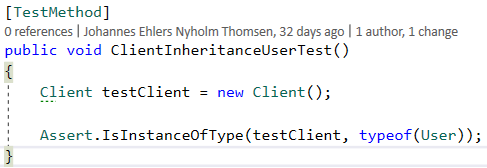
\includegraphics[width=\textwidth]{TestEksempelInheritance.png}
    \label{fig:TDD}
\end{figure}

TDD fungerede rigtig godt for os i de to første sprints, hvor programmets grundstruktur i domæne og applikationslagene blev skabt.
Da vi alle stadig er nye og uerfarne programmører, har vi været nød til at refaktorere koden af flere omgange.
Der har det været en uvurderlig gevinst, at vi nemt har kunne se, om vi har mistet funktionalitet i vores program eller ej.

I den sidste sprint må vi dog indrømme, at vi gik bort fra TDD pga. tidspres.
Det gjorde det dog meget sværere at debugge vores funktionalitet med tråde, og i retrospekt ville vi nok have sparet tid på også at bruge TDD til udvilkingen af dette.

\subsection{Lagdeling}
\label{lagdeling}

Inden vi begyndte at udvikle progammet havde udviklingsgruppen en diskussion om, hvordan vi ønskede at lagdele vores program.
Vi blev enige om at bruge en trelagsdeling
En streng lagdeling betyder, at et lag kun kender til og kan tale med laget lige under sig.
I en afslappet lagdeling kan et lag derimod kalde lag, der ligger flere lag under sig.\cite{larman}

Normalt kører man en afslappet lagdeling i informationssystemer, og en streng lagdeling i netværksprotokoller.
Ligegyldigt om man kører en afslappet eller streng lagdeling vil UI laget ikke kalde ens domænelag direkte, medmindre man ikke har et applikationslag.
Et applikationslag er ikke altid nødvendigt, men vi har valgt at have et, da programmet er komplekst nok til, at vi ikke kun kan have én softwareklasse til at håndtere programmets tilstand.\cite{larman}

Som det kan ses på figur \ref{fig:pakkediagram} har vi 4 lag: et UI lag, et applikationslag, et domænelag og et persistenslag.
Vi har en afslappet lagdeling, da det kan ses, at vores applikationslag både kalder domænelaget og persistenslaget.

For at sikre vores lagdeling har vi valgt at have lagene som selvstændige projekter.
Dette betyder, at hvert lag ligger i sit ejet namespace, og dermed gør det nemt at se, præcis hvilke lag et givent lag kender til.
Vores UI er en WPF-applikation, applikationslaget, domænelaget og persistenslaget er 2 klassebiblioteker.

\subsection{Designmønstre}
\label{designmoenstre}
Designmønstre hjælper programmører med at løse problemer, som andre har løst tidligere.
Når en person har fundet en god og genbrugelig løsning til et problem, er der ikke nogen grund til, at vi skal bruge tid på at opfinde den dybe tallerken igen.

Vi har i vores program gjort brug af flere designmønstre, som vi vil præsentere i dette afsnit.

\subsubsection{Facade}
\label{facade}

Idéen med en facade er at give en samlet snitflade for flere snitflader i et undersystem.
I stedet for at du som kunde i en restaurant, går ud og spørger hver enkelt kok, hvad han kan tilberede af retter, får du et menukort, hvor du kan se de retter, som restauranten tilbyder.

Vi bruger en facade mellem vores applikationslag og vores UI-lag, da UI-laget ikke behøver vide noget om, hvordan vores applikationslag ser ud, men blot skal vide, hvilken funktionalitet laget tilbyder.
Dette giver os en svag kobling mellem de to lag, og derved kan vi nemt ændre på applikationslaget uden at skulle bekymre os om, hvordan det påvirker UI-laget.\cite{gangoffour}
På figur \ref{fig:pakkediagram} kan det ses, at alle klasser i UI'et går igennem vores Controller klasse.

Vi har valgt at implementere denne facade som en controller, hvilket vil blive beskrevet nærmere i afsnit \ref{controller}.

\subsubsection{Singleton}
\label{singleton}

En singleton er en klasse, der kun har én instans og har et globalt tilgangspunkt for klassen.
Singletonmønstret giver mening, da der findes softwareklasser, hvor der kun må findes én eneste udgave af klassen.
Vores system skal kun have én kundeliste og kun én liste over behandlere, derfor er de implementerede som singletons.

Singletonmønstret har flere fordele: kontrolleret adgang til klassens ene instans.
Undgå rod i namespacet ved ikke at have det som globale variable.
Hvis man ændrer mening, og det ikke længere skal være en singleton, er det simpelt at redigere koden, så klassen tillader at blive instantieret flere gange. Faktisk kan man med singleton mønstret bestemme præcis hvor mange instanser af en klasse, som man ønsker.

På figur \ref{code:singleton} kan vores implementation af singletonmønstret ses.

Vi har flere klasser, der implementerer singletonmønstret: alle vores repositories er singletons.
Derfor burde vi have implementeret et singleton interface eller en abstract singleton klasse, som de andre singletons kunne arve fra.

\begin{figure}[h]
    \caption{PractitionerRepo's implementering af singletonmønstret}
    \centering
        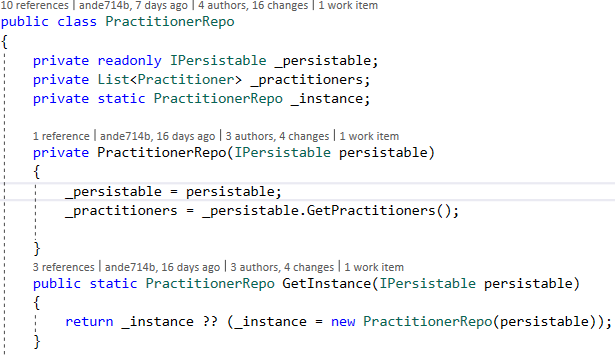
\includegraphics[width=\textwidth]{Singleton.png}
    \label{code:singleton}
\end{figure}

\subsubsection{Observer}
\label{observer}

Idéen med observermønstret er at skabe en fornuftig en-til-mange afhængigmed mellem objekter, så når et objekt ændrer tilstand får alle dens afhængige klasser en besked og opdateres automatisk.\cite{gangoffour}

Det bruges rigtig meget til at styre, hvordan et UI bliver opdateret, når programmet ændrer tilstand.

I C\# er der flere måder at implementere et observermønster: de mest udbredte måder er gennem 2 interfaces(et udgiver og et abonnent interface) eller ved hjælp af delegates.
I C\# findes en delegate, der hedder EventHandler, som normalt bruges, når man laver et observermønster vha delegates.

Som det kan ses på figur \ref{fig:ControllerObserverPattern} har vi implementeret vores observermønstre ved brug af EventHandler delegaten.
Vi har valgt at bruge delegates i stedet for interfaces, da vi så ikke behøver at lave og implementere to interfaces, men i stedet gør vi brug af værktøjer, der allerede eksisterer.
Derudover ville vi gerne få mere erfaring i at bruge delegates og events, da vi ikke har arbejdet lige så meget med det i løbet af året som med interfaces.

Som det kan ses på figur \ref{fig:ControllerObserverPattern} er vores Controller klasse både en udgiver og en abonnent.
Det er den nød til, da som beskrevet i afsnit \ref{facade}, er Controller en facade, og derfor kan vores UI ikke abonnere direkte ned til andre udgivere i vores applikationslag.


\begin{figure}[h]
    \caption{Controller observer mønster}
    \centering
        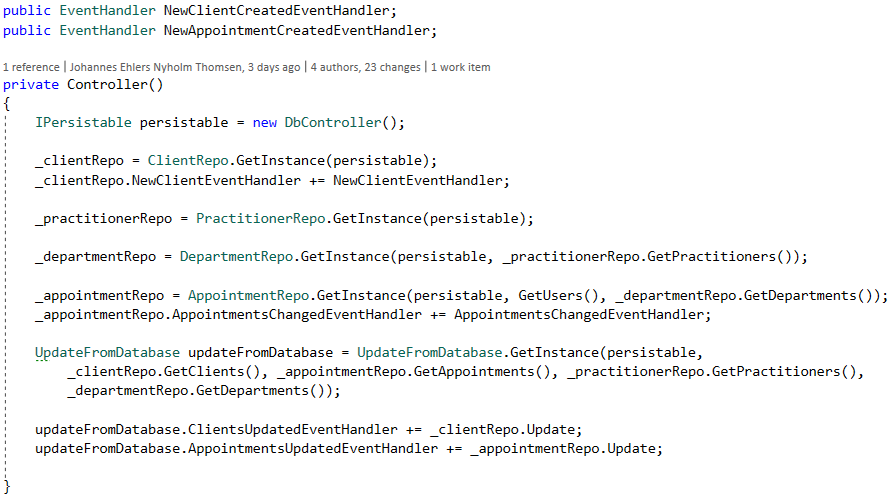
\includegraphics[width=\textwidth]{ControllerObserverPattern.png}
    \label{fig:ControllerObserverPattern}
\end{figure}

Vores UI abonnerer på vores controller, som abonnerer på vores appointmentrepo og clientrepo klasser.
På figur \ref{fig:ObserverObservermethod} kan det ses, at når controlleren får at vide, at der er sket en ændring i clientrepo eller appointmentrepo giver den sine abonnenter besked om det.
Vores LandingPage og CreateAppointment vinduer abonnerer på vores controller.
Det medfører, at når en aftale bliver lavet, opdateres aftaleoversigten på vores LandingPage.

\begin{figure}[h]
    \caption{Controller abonnentmetoder.}
    \centering
        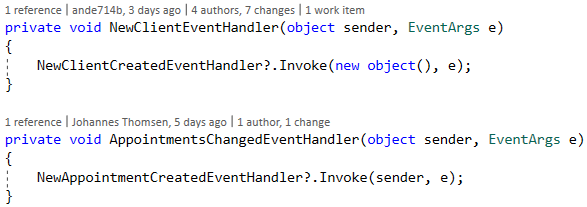
\includegraphics[width=\textwidth]{ObserverObservermethod.png}
    \label{fig:ObserverObservermethod}
\end{figure}

\subsection{Interfaces og nedarvning}

\subsection{Threads}

\subsection{Delegates og Lambdaudtryk}

\subsection{LINQ}

\subsection{GRASP}
\label{grasp}
GRASP står for General Responsibility Assignment Software Principles og er udgivet af Craig Larman.\cite{larman}

Principperne skal hjælpe med at skrive kode af høj kvalitet, så det skal være nemt at vedligeholde, udvide, og det skal være modulært.

Vi har arbejdet med 5 GRASP principper: Creator, Information 
Expert, Low Coupling, High Cohesion og Controller.

\subsubsection{Creator}

Creator princippet hjælper os med at bestemme, hvilken klasse skal have ansvaret for at lave en anden klasse.
Larman giver os flere betingelser for, hvornår klasse A skal lave klasse B:

\begin{itemize}
    \item A indeholder B
    \item A samler B
    \item A har initialiseringsdataerne for B
    \item A optager B
    \item A nøje bruger B
\end{itemize}

Ifølge disse principper betyder det, at vores controller også kunne lave blandt andet vores aftaleklasse, se figur \ref{fig:controllerCreator}, da den indeholder alt den nødvendige data til at instantiere klassen.
Det vil dog bryde med single responsibility princippet, som vi behandler i afsnit \ref{SRP}.
Derfor er det appointmentRepo klassen, der har ansvaret for at lave et nyt appointment objekt, da denne samler appointment objekter.
Som det kan ses på figur \ref{fig:controllerCreator} sender controlleren informationen videre ned til AppointmentRepo objektet, som så laver et Appointment objekt.

\begin{figure}[h]
    \caption{Controller CreateAppointment metode}
    \centering
        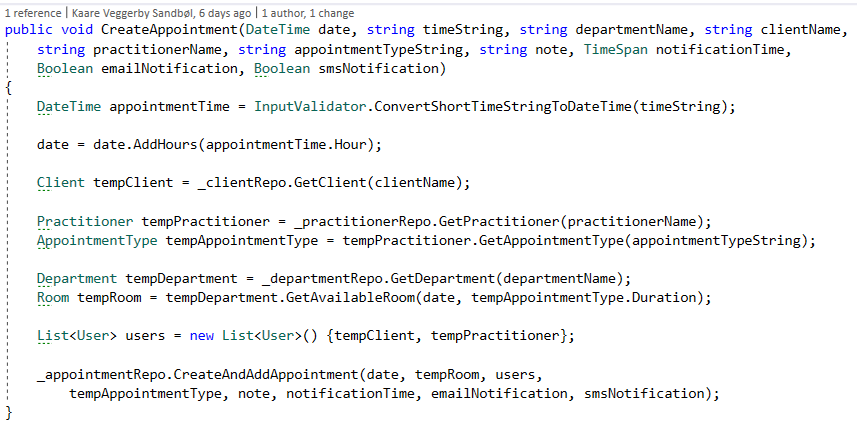
\includegraphics[width=\textwidth]{CreateAppointmentCreator.png}
    \label{fig:controllerCreator}
\end{figure}

\subsubsection{Information Expert(IE)}
IE princippet er et princip, der skal hjælpe os med single responsibility princippet.

IE siger, at den klasse, der har den nødvendige information til at udføre en handling, skal have ansvaret for at udføre den handling.

Da practitioner klassen indeholder den information, der skal bruges til at finde ud af, hvornår en practitioner har en ledig tid, er det derfor den klasse der skal udføre den handling, se figur \ref{fig:informationexpert}.
De to hjælpemetoder kan ses i bilagene på figur \ref{bilag:informationexpert}.

\begin{figure}[h]
    \caption{IE eksempel i practitioner klassen}
    \centering
        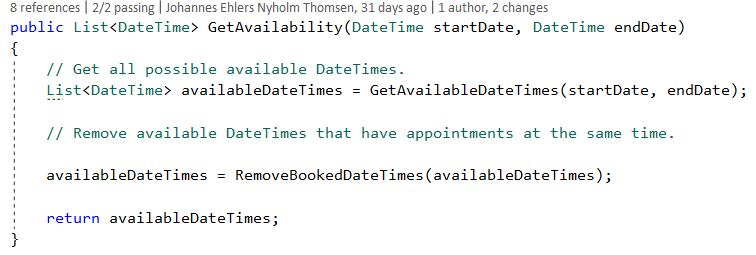
\includegraphics[width=\textwidth]{IEEksempel.png}
    \label{fig:informationexpert}
\end{figure}

\subsubsection{Controller}
\label{controller}
Vi gør brug af en controller til at facilitere kald fra UI'et, der kræver kald ned i applikations- og domænelaget.
Dette betyder, at vi indkapsulerer en systemoperation.
En systemoperation er noget, som en bruger af systemet ønsker at opnå, f.eks at booke en ny aftale, altså de operationer, som vises i et SSD.

Vi opnår så systemoperationen ved, at controlleren kalder de nødvendige metoder i resten af systemet.

Da vi, som nævnt i afsnit \ref{lagdeling}, har et applikationslag er det oplagt at bruge en controller til netop at give os det ønskede lag mellem UI og domæne.

Vores controller er også en facade mellem UI- og applikationslagene, se afsnit \ref{facade}.

\subsection{SOLID}
\label{solid}

SOLID er en samling af principper givet af Robert C. Martin.
På samme måde som GRASP skal SOLID principperne hjælpe en programmør med at skrive kvalitetskode.

Vi er blevet undervist i single responsibility i løbet af dette år.

\subsubsection{Single responsibility princip(SRP)}
\label{SRP}

Idéen med SRP er, at en klasse må kun have ét ansvar.\cite{solid}

En fare ved at bruge en controller er, at den godt kan komme til at have mere end et ansvar.
Det har vi forsøgt at være meget opmærksomme på, hvilket også er grunden til, at vi har klasser som InputValidator klassen og DateTimeCalculator klassen.
Begge klasser er i bund og grund metodebiblioteksklasser, da de kun indeholder statiske metoder.
InputValidator klassen sikrer, at input fra brugeren er gyldige inputs, inden de bliver brugt af resten af systemet.
Et eksempel af dens brug kan ses på figur \ref{fig:InputValidator}.

Det kan dog ses på figur \ref{fig:controllerCreator}, at det ikke er lykkedes os helt at overholde SRP for controller klassen, da dens CreateAppointment metode også går ind og samler oplysninger fra andre objekter, og giver dem videre til appointmentrepo objektet.

Den har altså nu mere end et ansvar: den faciliterer ikke kun samarbejde mellem UI og applikationslag, men samler også informationer fra andre klasser i applikationslaget.

\begin{figure}[h]
    \caption{Controllers brug af InputValidator metoder}
    \centering
        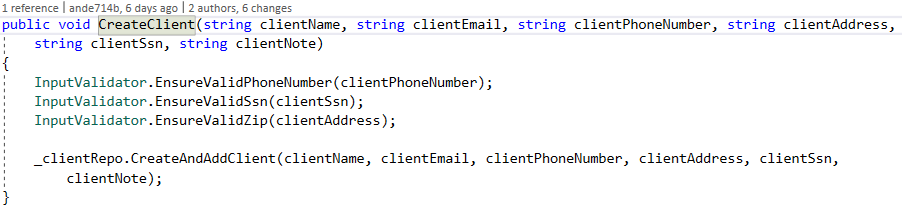
\includegraphics[width=\textwidth]{InputValidator.png}
    \label{fig:InputValidator}
\end{figure}

En af gevinsterne ved at bruge SRP er, at man får høj samhørighed i ens program.

Man skulle tro, at SRP og høj samhørighed bryder med en anden idé, der hedder lav kobling.     
Idéen med lav kobling eller low coupling er, at klasserne i ens software skal være så uafhængige af andre klasser som muligt.

Lav kobling betyder dog ikke, at et program har ingen kobling.
Hele filosofien bag objektorienteret programmering er, at man repræsentere ens problem med klasser, og hvordan de klasser taler sammen.
Men hvis man forsøger at reducere kobling så meget som muligt gør det det nemmere at udvide og ændre ens program.

På figur \ref{fig:DCD} kan det ses, hvor mange af vores klasser kender til hinanden.